\subsection{Objektorientierung}
\label{sec:Kap-3.2.1}

Die objektorientierte \textbf{Modellierung} hat ihren Ursprung in den Konzepten und Prinzipien der objektorientierten \textbf{Programmierung}. Die erste objektorientierte Programmiersprache war Simula67, die Ole-Johan Dahl und Kristen Nygaard in den 1960er Jahren entwickelten. Aus Simula67 stammt das für die Objektorientierung zentrale Grundkonzept von Klassen und Objekten. Die seit den 1970er Jahren von Adele Goldberg, Dan Ingalls und  Alan Kay entwickelte Programmiersprache Smalltalk \cite{gol83} ist damit zwar nicht die erste objektorientierte Programmiersprache; sie gilt trotzdem heute als Ursprung der Objektorientierung, da sie in Simula67 angelegte Konzepte, wie Datenkapselung und Vererbung, konsequent objektorientiert aus\-arbeitete und um neue Konzepte wie Polymorphie und dynamisches Binden ergänzte, die heute zu den zentralen Charakteristika der Objektorientierung zählen. Seit Ende der 1980er Jahre lösten objektorientierte Programmiersprachen zunehmend andere Arten von Programmiersprachen (wie die strukturierte Programmierung) ab. 

Die 
\marginline{Ziele}
objektorientierte Programmierung erhob den Anspruch, die Komplexität von Softwareentwicklung reduzieren zu können, Software besser testbar, besser wartbar und einfacher erweiterbar zu machen und die Wiederverwendung von Konzepten und Programmcode zu fördern. Dazu beinhaltete sie verschiedene (Entwurfs)Prinzipien wie Datenkapselung, Geheimnisprinzip, Modularisierung, Vererbung, Polymorphie und Abstraktion. Die heute verbreiteten objektorientierten Programmiersprachen weichen von der durch Smalltalk begründeten reinen Lehre der Objektorientierung allerdings in einigen Aspekten ab (\zb primitive Datentypen). Zudem zwingen sie die Programmierer unterschiedlich strikt zur Einhaltung dieser objektorientierten Prinzipien. Das hat zur Folge, dass es auch mit objektorientierten Programmiersprachen durchaus möglich ist, nicht-objektorientiert zu implementieren. 

Die  Basis der Objektorientierung ist das \textit{Objekt}.
\marginline{Objekt}
Ein Objekt in einer Software ist eine Einheit aus Daten und Operationen, die auf diesen Daten arbeiten. Damit unterscheidet sich die Objektorientierung von der zuvor verbreiteten strukturierten Programmierung, wie sie zum Beispiel mit Programmiersprachen wie Pascal und C verbunden ist. In der strukturierten Programmierung werden Daten und Operationen als getrennte Einheiten behandelt. Die Programmierer der Software müssen darauf achten, dass die Operationen auf den richtigen Daten arbeiten. Nach der reinen objektorientierten Lehre dagegen arbeiten auf den Daten eines Objekts nur seine eigenen Operationen. 

Zur Laufzeit der Software existiert eine (durch den Programmcode definierte) veränderliche Menge von Software-Objekten, die in Beziehungen zueinander stehen und miteinander interagieren.

Neben  der Kapselung von Daten und Operationen in einem Objekt besteht die zentrale Idee der Objektorientierung in der engen Orientierung an der Realwelt. 
\marginline{Realweltbezug – das zentrale Konzept der Objekt\-orientierung}
Die Objektorientierung versucht Strukturen der Realwelt in Software nachzubilden. Dafür werden die Objekte der Software anhand der Merkmale und des Verhaltens von Objekten des zu modellierenden Realweltausschnitts (Domäne) konstruiert. Dabei ist es wichtig, geeignete Abstraktionsebenen zu wählen: Für die Konstruktion der Software-Objekte werden nur diejenigen Merkmale der Realwelt-Objekte berücksichtigt, die für den Anwendungszweck des zukünftigen Softwareprodukts relevant sind. 

\begin{figure}[h!]
	\centering
	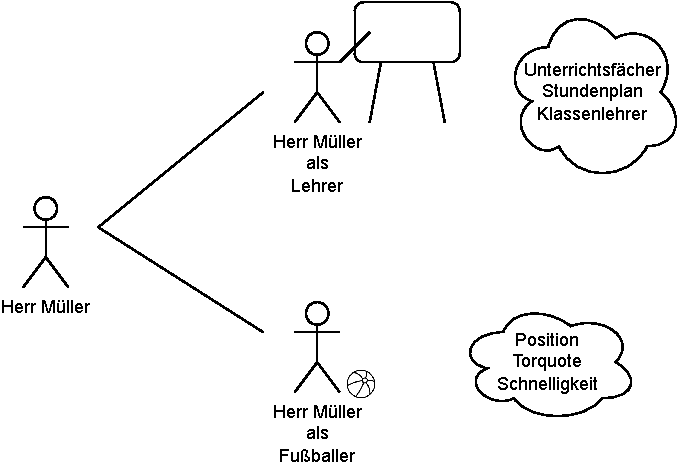
\includegraphics{Bilder/Kapitel-3/mueller_lehrer_fussballer.pdf}
	\caption{Herr Müller als Lehrer und als Fußballer}
	\label{fig:mueller_lehrer_fussballer}
\end{figure}

Abbildung~\ref{fig:mueller_lehrer_fussballer} zeigt 
\marginline{das Prinzip der Abstraktion}
links die Realwelt-Person Herrn Müller – bzw. ein Strichmännchen, von dem wir so tun, als sei es Herr Müller. Herr Müller ist von Beruf Lehrer und in seiner Freizeit begeisterter Fußballer. Angenommen, wir möchten eine Schul\-verwal\-tungs\-soft\-ware entwickeln, in der der Realwelt-Lehrer Herr Müller als Software-Objekt Lehrer Müller vorkommen soll. In diesem Fall würden uns Merkmale des Realwelt-Menschen Herrn Müller interessieren, die mit seinem Lehrerberuf zu tun haben, zum Beispiel welche Fächer unterrichtet er, wie sieht sein Stundenplan aus, ist er Klassenlehrer? Wenn wir statt einer Schulverwaltungssoftware ein Wettportal für Fußballwetten entwickeln wollten, würde uns an Herrn Müller dagegen interessieren, auf welcher Position er spielt, welche Torquote er hat und wie hoch seine Schnelligkeit ist. 

Bei der Konstruktion von Software-Objekten geht es darum, die für die zu erstellende Software relevanten Charakteristika von Realwelt-Objekten abzubilden und von allen anderen Merkmalen der Realwelt-Objekte zu abstrahieren. Wie das konkret geht, sehen wir uns in Kapitel~\ref{sec:Kap-4} an. Zunächst beschäftigt uns hier das Domänenmodell -- das alle diese modellierten Realwelt-Objekte später umfasst -- nochmal als Ganzes.